\newpage
\chapter{Desenvolvimento}
\label{ch:desenvolvimento}

\par Este capítulo aborda cada uma das etapas do processo de desenvolvimento dos recursos assistivos e implementação da biblioteca ICan.js. Os processos detalhados neste capítulo são apresentados de forma geral na Figura \ref{figure:fluxmethod}.

\image{0.17}{imagens_arquitetura/fluxo_de_desenvolvimento_icanjs.png}{Fluxo de desenvolvimento do projeto}{figure:fluxmethod}{Produção do autor}

\par Como apresentado na Figura \ref{figure:fluxmethod}, inicialmente fez-se a aquisição das imagens de Libras (a), a etapa de processamento, geração do modelo e distribuição do mesmo é feita (b), por fim, cria-se a arquitetura da biblioteca e realiza-se a implementação dos recursos assistivos (c).

\section{Arquitetura da biblioteca}

\par A arquitetura da biblioteca, como apresentado anteriormente, foi desenvolvida após as etapas de processamento e criação dos modelos, porém para a boa compreensão do desenvolvimento deste trabalho, inicialmente é feito a apresentação da biblioteca e sua arquitetura, o que possibilita posteriormente a fácil ligação de cada um de seus módulos e funções com as etapas anteriores. 

\par A arquitetura do ICan.js, foi criada seguindo a estrutura apresentada em \cite{tensorflowjs2019}, desta forma, a arquitetura é separa em conjuntos de funcionalidades, o que permite um desenvolvimento organizado e uma utilização facilitada. Neste caso, os conjuntos são nomeados \textit{Core} e \textit{Common}, estes que são construídos sobre as funcionalidades disponibilizadas pelo Tensorflow.js (TFJS) e P5.js respectivamente, como apresentado na Figura \ref{figure:icanjsarch}.

\image{0.2}{imagens_arquitetura/arquitetura_camadas_icanjs.png}{Arquitetura do ICan.js}{figure:icanjsarch}{Produção do autor}

\par O conjunto \textit{Core} é responsável por disponibilizar funcionalidades base para o desenvolvimento dos recursos assistivos, como o acesso a \textit{webcam} dos usuários, os modelos de regressão e também os modelos de rede neural, podendo estes serem carregados da \textit{API} de distribuição ou mesmo do próprio TFJS. Boa parte de suas funcionalidades foram implementadas utilizando o TFJS, e todo seu desenvolvimento foi feito através do ambiente Node.js, o que permitiu o desenvolvimento organizado e estruturado através de classes. O diagrama de classes da camada \textit{Core} é apresentado na Figura \ref{figure:icanjscoredc}.

\image{0.6}{imagens_arquitetura/diagrama_de_classe_core.png}{Diagrama de classes da camada \textit{Core}}{figure:icanjscoredc}{Produção do autor}

Já a camada \textit{Common} utiliza as funcionalidades do \textit{Core} junto a biblioteca P5.js para a criação dos recursos assistivos propriamente ditos, estes que tem sua utilização disponibilizada através da utilização de simples funções, como apresentado na Figura \ref{figure:icanjsrelacoes}.

\image{0.7}{imagens_arquitetura/arquitetura_expandida_icanjs.png}{Relação entre cada uma das camadas}{figure:icanjsrelacoes}{Produção do autor}

\par Para a exposição de cada um dos componentes nos conjuntos apresentados na Figura \ref{figure:icanjsrelacoes}, as seções seguintes apresentam as etapas do desenvolvimento de cada um dos recursos assistivos e os componentes relacionados a cada um destes.

% ToDo: Inserir um diagrama que explica a relação de todos os componentes da biblioteca, isto deixa a coisa mais clara
% \par \textbf{AQUI SERÁ ADICIONADO UM DIAGRAMA CONTENDO A RELAÇÃO DE TODOS OS COMPONENTES DO PROJETO}

% \textbf{EI! AQUI FALA DA ARQUITETURA GERAL DA COISA, MOSTRA A RELAÇÃO ENTRE AS FUNCIONALIDADES, O DIAGRAMA DE CLASSE DA CAMADA CORE, PARA TRAZER MAIS INFORMAÇÕES AO LEITOR SOBRE O QUE FOI FEITO....}

\section{Tradução de Libras para Texto}

\par Este recurso assistivo permite a interação dos usuários com deficiência auditiva a páginas da \textit{web} através de gestos de Libras. As etapas descritas nas subseções abaixo são apresentadas na Figura \ref{figure:fluxmethod}.

\subsection{Aquisição dos dados}

\par O grande desafio para o desenvolvimento deste recurso assistivo, foi a base de dados, já que, atualmente não há uma base de dados de Libras disponível publicamente \cite{Magalh2018}, de modo a ser necessário a criação de uma base de dados para o presente trabalho.

\par A seleção dos gestos que fazem a composição da base de dados foi feita seguindo um critério de identificação, neste é necessário que o gesto possa ser identificado com apenas um \textit{frame}, ou seja, apenas uma imagem é o suficiente para a identificação do gesto, o que torna a rede neural aplicada mais simples quando comparada a uma classificação que leva em consideração múltiplas imagens. Desta forma os gestos selecionados foram descritos com esta característica de identificação em \cite{Magalh2018}, sendo eles (a) Amigo, (b) Desculpa, (c) Telefone, estes apresentados na Figura \ref{figure:gestos_selecionados}.

\begin{figure}[H]
    \centering
    \subfloat[Amigo]{{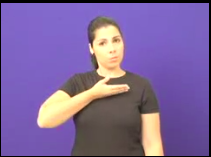
\includegraphics[height=3cm, width=5cm]{src/images/amigo.png}}}%
    \qquad
    \subfloat[Desculpa]{{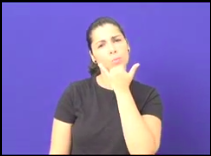
\includegraphics[height=3cm, width=5cm]{src/images/desculpa.png} }}%
    \qquad
    \subfloat[Telefone]{{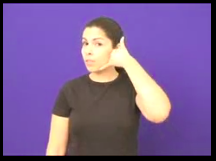
\includegraphics[height=3cm, width=5cm]{src/images/telefone.png} }}%
    \qquad
    \caption{Gestos selecionado para o conjunto de dados}%
    \label{figure:gestos_selecionados}%
    \fonte{Adaptado de \citeonline{dicioLibras2011}}
    % \fonte{Produção do autor} % Adaptado de Dicionário de Libras
\end{figure}

\par Para a aquisição dos dados, foi desenvolvido uma ferramenta \textit{desktop} multiplataforma na linguagem Python, com a utilização das bibliotecas PyQt e OpenCV. O fluxo de funcionamento da ferramente é apresentado na Figura \ref{figure:sistema_aquisicao_fluxo}.

\image{0.55}{ferramenta_coleta_de_dados/ferramenta_de_aquisicao_fluxo.png}{Tela inicial da aplicação de aquisição de dados}{figure:sistema_aquisicao_fluxo}{Produção do Autor}

\par Assim como apresentado na Figura \ref{figure:sistema_aquisicao_fluxo}, o sistema ao ser iniciado, apresenta informações gerais para o usuário e então já começa o processo de coleta de dados, neste, exemplos dos gestos a serem reproduzidos pelo usuário são exibidos, juntamente a imagem do próprio usuário (Figura \ref{figure:sistema_aquisicao}), além de uma barra de porcentagem para indicar ao usuário seu processo geral na aquisição das imagens.

% \textbf{O MAGONES RECOMENDOU A MUDANÇA DESTA IMAGEM!}
\image{0.60}{recurso_assistivo_escrita_com_gestos/tela_programa_aquisicao_de_dados.png}{Tela inicial da aplicação de aquisição de dados}{figure:sistema_aquisicao}{Produção do Autor}

\par No total, o sistema captura 60 imagens, sendo 20 para cada um dos gestos, em cada uma das imagens capturadas é aplicado uma operação de redimensionamento, isto para que, todas as imagens ao final do processo tenham a dimensão 224x224x3, independente do tamanho original capturado. Após a aquisição das 60 imagens o programa compacta as imagens salvas e às envia por \textit{email}.

% por \textit{email}

% \par Como apresentado na Figura \ref{figure:sistema_aquisicao}, o sistema de aquisição de imagens demonstra exemplos dos gestos que devem ser reproduzidos pelo usuário, uma barra de progresso, e botões para começar e recomeçar a captura das imagens do usuário e também para saber mais sobre o projeto.

% \par Este sistema captura 60 imagens, sendo 20 de cada um dos gestos, em cada uma das imagens capturadas é aplicado uma operação de redimensionamento, isto para que, todas as imagens tenham as dimensões 224x224x3, já que esta é a dimensão aceita pelo \textit{Mobilenet}, o modelo que será retreinado com os dados que estão sendo coletados. Após a aquisição das 60 imagens o programa cria um arquivo no formato zip e o envia para um \textit{email} criado para o armazenamento dos dados.

\par O programa foi distribuído e ao final houveram 12 colaboradores, criando assim um conjunto com 720 imagens, com quantidades igualmente distribuídas para cada gesto. Este conjunto de dados foi separado em duas partes, a primeira, com imagens de 11 colaboradores, para o treino e teste do modelo de rede neural, e a segunda para a validação, separando 1 colaborador.

\subsection{Pré-processamento dos dados}

\par Durante a aquisição das imagens, nenhuma restrição foi emposta aos colaboradores para tornar o identificador de imagens o mais geral possível, assim uma etapa de validação de cada uma das imagens teve de ser realizada para garantir que, cada imagem representa o gesto ao qual é indicado, o que resultou na remoção de algumas imagens. Este processo foi realizado nos dois grupos de dados criados. A Figura \ref{figure:plot_qtd_apos_filtro_por_grupo} apresenta a relação da quantidade de imagens com cada um dos gestos após a validação realizada nos grupos de dados. 

\image{1.0}{imagens_pre_processamento_de_dados/plot_grupos_dados_pre_processamento.jpeg}{Quantidade de imagens por gesto após filtragem em cada grupo}{figure:plot_qtd_apos_filtro_por_grupo}{Produção do Autor}

\par Após a filtragem, o grupo de dados para treino e teste foi dividido, ficando 80\% dos dados para treino e 20\% para teste. Este processo foi criado utilizando a biblioteca sklearn, e o código é apresentado na Figura \ref{figure:split_train_test_data}.

\begin{figure}[H]
    \centering
    \begin{lstlisting}[language=Python]
from sklearn.model_selection import train_test_split

x, y = [], []

for collaborator_dir in os.listdir():
    files = os.listdir(collaborator_dir)

    x.extend(files)
    y.extend(np.repeat(collaborator_dir, len(files)))

x_train, x_test, y_train, y_test = train_test_split(x, y, test_size=0.20, random_state=992)    
\end{lstlisting}
    \caption{\textit{Script} de separação dos dados (Treino X Teste)}
    \fonte{Produção do autor}
    \label{figure:split_train_test_data}
\end{figure}

\par Veja que, das linhas 5 a 9, a referência do arquivo de cada um dos colaboradores é colocada dentro de listas, cada uma delas representando respectivamente, o arquivo e a classe a qual o arquivo representa, após isto, na linha 11, as listas são divididas em treino e teste.

% \par Veja que, para cada colaborador há um diretório contendo as imagens coletadas, estes diretórios são percorridos e cada imagem e o gesto que a mesma representa são salvos em uma lista, que posteriormente é dividida em listas de treino e teste com a função \textitbf{train\_test\_split}.

\par Com a divisão realizada, cada uma das imagens divididas em treino e teste são movidas para os diretórios de seus respectivos tipos (Figura \ref{figure:move_splitted_data}).

\begin{figure}[H]
    \centering
    \begin{lstlisting}[language=Python]
def move_data(x_data: list, y_data: list, typeof: str) -> None:
    for xt, yt in zip(x_data, y_data):
        src = os.path.join(yt, xt)
        dst = os.path.join(typeof, yt, xt)
        
        copyfile(src, dst)
\end{lstlisting}
    \caption{Função para movimentação dos arquivos de Treino e Teste}
    \fonte{Produção do autor}
    \label{figure:move_splitted_data}
\end{figure}

\par A função da Figura \ref{figure:move_splitted_data}, recebe a lista com as referências dos arquivos e classes e então copia os arquivos para o diretório onde será utilizado no treinamento e validação.

\par Com a finalização da separação dos dados, as quantidades de imagens nos conjuntos de treino/teste podem ser vistas na Figura \ref{figure:qtd_imagem_treino_teste}.

\image{0.80}{quantidade_de_imagem_por_tipo.jpeg}{Quantidade de imagen de treino e teste}{figure:qtd_imagem_treino_teste}{Produção do Autor}

% ToDo (20/04/2019) Verificar a explicação do Data Augmentation
\par Poucas imagens podem ser um problema para a generalização do modelo, mesmo levando em consideração o retreino do \textit{MobileNet} que será feito, assim será aplicado no conjunto de teste o \textit{Data Augmentation}, que através de modificações nas imagens existentes faz a criação de novas imagens. A técnica foi aplicada somente no conjunto de treino/teste.

\par Para a aplicação do \textit{Data Augmentation} utilizou-se a biblioteca Augmentor. Nesta foi feito a definição das probabilidades de ocorrência de um conjunto de modificações nas imagens durante o processo de aplicação das modificações.

% \par Neste trabalho, o \textit{Data Augmentation} foi realizado com o auxílio do \textit{Augmentor}, uma biblioteca Python que permite a criação de um \textit{Pipeline} de alterações baseado em probabilidade, assim atribui-se para cada alteração que pode ser aplicada na imagem uma probabilidade de ocorrência, e então o \textit{Augmentor} com base nas probabilidades aplica uma ou várias alterações na base de imagens. 

\par A Figura \ref{figure:pipeline_data_augmentation} apresenta todas as alterações que podem ser aplicadas nas imagens durante o processo de aplicação das modificações.

\image{1.0}{recurso_assistivo_escrita_com_gestos/pipeline_de_geracao_de_imagens.jpeg}{Alterações aplicadas no \textit{Pipeline} do \textit{Data Augmentation}}{figure:pipeline_data_augmentation}{Produção do Autor}.

\par O trecho de código apresentado na Figura \ref{figure:dataaugmentation} demonstra como é a implementação do processo de alterações nas imagens vistos na Figura \ref{figure:pipeline_data_augmentation}.

\begin{figure}[H]
    \centering
    \begin{lstlisting}[language=Python]
import Augmentor

p = Augmentor.Pipeline('gestos_editados/treino')

p.random_distortion(probability=0.5, grid_height=3, grid_width=3, magnitude=2)

p.skew_left_right(probability=0.3, magnitude=0.7)
p.skew_corner(probability=0.4, magnitude=0.5)

p.sample(700)
    \end{lstlisting}
    \caption{Trecho do \textit{Script} de \textit{Data Augmentation}}
    \fonte{Produção do autor}
    \label{figure:dataaugmentation}
\end{figure}

\par Na linha 3 cria-se a instância de um processo de alterações, referenciando o diretório onde estão as imagens que são modificadas para a geração das novas imagens. Da linha 5 a 8 são feitas definições de algumas modificações a serem aplicadas nas imagens, e por fim, na linha 10, 700 imagens são geradas através deste processo.

% \par Veja que, cria-se inicialmente uma instância de \textit{Pipeline} indicando apenas o diretório das imagens de treino, e então todas as possíveis modificações são declaradas na instância de \textit{Pipeline} e junto a cada uma delas uma probabilidade. No fim, é indicado que o total de imagens gerado deve ser 700.

\par A Figura \ref{figure:gestos_gerados_no_pipeline} apresenta exemplos de imagens geradas com as diferentes modificações indicadas no código.

\begin{figure}[H]%
    \centering
    % \subfloat[]{{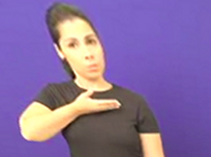
\includegraphics[height=3cm, width=5cm]{src/images/imagens_alteradas_pelo_pipeline/amigo_1.png}}}%
    % \qquad
    \subfloat[]{{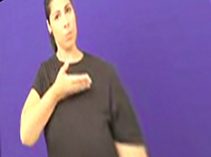
\includegraphics[height=3cm, width=5cm]{src/images/imagens_alteradas_pelo_pipeline/amigo_2.png}}}%
    \qquad
    % \subfloat[]{{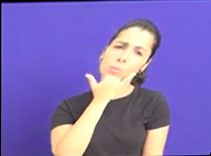
\includegraphics[height=3cm, width=5cm]{src/images/imagens_alteradas_pelo_pipeline/desculpa_1.png}}}%
    % \qquad
    \subfloat[]{{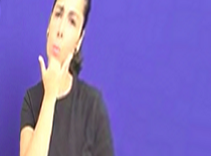
\includegraphics[height=3cm, width=5cm]{src/images/imagens_alteradas_pelo_pipeline/desculpa_2.png}}}%
    \qquad
    \subfloat[]{{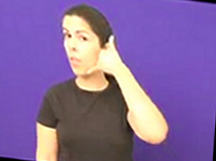
\includegraphics[height=3cm, width=5cm]{src/images/imagens_alteradas_pelo_pipeline/telefone_1.png}}}%
    \qquad
    % \subfloat[]{{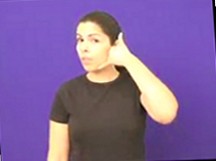
\includegraphics[height=3cm, width=5cm]{src/images/imagens_alteradas_pelo_pipeline/telefone_2.png}}}%
    % \qquad
    \caption{Exemplos de imagens geradas pelo processo de modificação}%
    \label{figure:gestos_gerados_no_pipeline}
    \fonte{Produção do autor} 
\end{figure}

\par Após a aplicação do \textit{Data Augmentation} o conjunto de treino/teste passou a ter 700 imagens, a Figura \ref{figure:plot_qtd_apos_dataaugmentation} mostra este valor distribuído por gesto.

\image{1.0}{imagens_pre_processamento_de_dados/quantidade_de_gestos_apos_data_augmentation.jpeg}{Quantidade de imagens por gesto com \textit{Data Aumentation}}{figure:plot_qtd_apos_dataaugmentation}{Produção do Autor}

\subsection{Treinamento da Rede Neural Convolucional}

\par O modelo de CNN utilizado neste recurso assistivo foi o \textit{MobileNet}, disponibilizado pela biblioteca Keras, com os pesos sinápticos obtidos através do treinamento da rede no conjunto de dados ImageNet \cite{Russakovsky2015}, que possui 1.28 milhões de imagens de 1000 classes.

\par Inicialmente, cria-se o modelo \textit{MobileNet}, com os pesos do conjunto ImageNet, porém, este modelo não possui as camadas de classificação, desta forma aplica-se as camadas finais e de classificação no modelo carregado. A Figura \ref{figure:criacao_do_modelo} apresenta o trecho de código. Na linha 2 é criado a instância do \textit{MobileNet}, nas linhas 5 e 6 cria-se a camada de saída, com um filtro, as linhas 9, 10, e 11, são adicionadas camadas totalmente conectadas, por fim, nas linhas 14 e 17, é criado o classificador e um novo modelo de MobileNet é gerado, respectivamente.

\begin{figure}[H]
    \centering
    \begin{lstlisting}[language=Python]
# Criando o modelo que será retreinado
mobile_net = MobileNet(input_shape=(224, 224, 3), weights='imagenet', include_top=False)

# Configurando o novo topo da rede neural
model_top = mobile_net.output
model_top = GlobalAveragePooling2D()(model_top)

# Adicionando mais camadas no topo
model_top = Dense(1024, activation='relu')(model_top)
model_top = Dense(1024, activation='relu')(model_top) 
model_top = Dense(512, activation='relu')(model_top)

# Classificador
model_top_classifier = Dense(3, activation='softmax')(model_top)

# Gerando novo modelo
new_mobile_net = Model(inputs=mobile_net.input, outputs=model_top_classifier)
    \end{lstlisting}
    \caption{Trecho de código para a criação do modelo}
    \fonte{Produção do autor}
    \label{figure:criacao_do_modelo}
\end{figure}

\par Neste trabalho aplicou-se a técnica de transferência de aprendizado no \textit{MobileNet}, assim foram selecionados para o treinamento todas as camadas após o segundo bloco de convolução, aproveitando assim as especifidades dos blocos até o segundo e buscando novas características nas camadas a frente. Desta maneira, a Figura \ref{figure:descongelamento_modelo} apresenta o trecho de código para criação do modelo. Na linha 1 todos os blocos de convolução após o segundo são postos para treinamento.

\begin{figure}[H]
    \centering
    \begin{lstlisting}[language=Python]
new_mobile_net = unfreeze_layers_from(new_mobile_net, 20)
    \end{lstlisting}
    \caption{Trecho de código da seleção dos blocos a serem treinados}
    \fonte{Produção do autor}
    \label{figure:descongelamento_modelo}
\end{figure}

\par Com a definição da camada de classificação e das camadas que serão retreinadas, o modelo é configurado para o treinamento através da definição das métricas, funções de otimização e perda que serão utilizados. O código na Figura \ref{figure:configuracao_do_modelo_para_treino} apresenta esta configuração do modelo.

\begin{figure}[H]
    \centering
    \begin{lstlisting}[language=Python]
new_mobile_net.compile(optimizer=Adam(lr=1e-3), \
        loss='categorical_crossentropy', metrics=['accuracy'])
    \end{lstlisting}
    \caption{Trecho de código da seleção dos blocos a serem treinados}
    \fonte{Produção do autor}
    \label{figure:configuracao_do_modelo_para_treino}
\end{figure}

\par Após as configurações, o treinamento do modelo foi realizado com 5 épocas, onde cada uma das épocas representa a quantidade de vezes em que a rede viu o conjunto de dados por completo. Este processo de treinamento foi realizado utilizando a plataforma Colab. A Figura \ref{figure:treinamento_do_modelo} apresenta o trecho de código de inicialização do treinamento.

\begin{figure}[H]
    \centering
    \begin{lstlisting}[language=Python]
new_mobile_net.fit_generator(train_generator,
                            steps_per_epoch=8,
                            epochs=5,
                            validation_data=test_generator,
                            validation_steps=2)

new_mobile_net.save('results/icanv2.h5')
    \end{lstlisting}
    \caption{Trecho de código do treinamento do modelo}
    \fonte{Produção do autor}
    \label{figure:treinamento_do_modelo}
\end{figure}

\par É apresentado na Figura \ref{figure:treinamento_do_modelo}, na linha 7 que, o modelo será salvo no formato H5, porém para a utilização deste modelo na biblioteca TFJS, faz-se necessário a conversão deste para o formato JSON, que é lido pelo TFJS. A conversão realizada na ferramenta \textit{tensorflowjs\_converter} é apresentada na Figura \ref{figure:conversao_do_modelo}.

\begin{figure}[H]
    \centering
    \begin{lstlisting}[language=Shell]
tensorflowjs_converter --input_format keras results/icanv2.h5 \
                                    results_tfjs/
    \end{lstlisting}
    \caption{Conversão de formato do modelo treinado}
    \fonte{Produção do autor}
    \label{figure:conversao_do_modelo}
\end{figure}

\par A utilização da ferramenta (Figura \ref{figure:conversao_do_modelo}) recebe o modelo salvo no formato H5 e o diretório onde o modelo no formato JSON será salvo.

% \par Com o modelo convertido este pode ser distribuído e consumido pela biblioteca TFJS.

% O modelo de CNN utilizado neste recurso assistivo é criado a partir da aplicação da técnica de aprendizado por transferência no modelo \textit{Mobilenet}.

%%%%% 16/03/2019
% Antes de continuar esta parte será necessário conseguir mais um colaborador, para que então sua imagem seja utilizada no conjunto de testes, para deixar mais coerente os resultados da rede.

% E a camada de convolução inicial foi alterada, desta forma, será utilizado da camada 10 em diante...

% Explicar que a camada 10 foi escolhida já que, quanto mais a frente mais específicos são as características escolhidas pela rede, ou seja, a base é mais genérica (Buscar uma referência)
%%%%%

% \par O modelo treinado é normalmente salvo no formato \textbf{H5}, porém neste caso, ele será convertido para um formato otimizado para \textit{web}, e que poderá ser consumido pelo TFJS.

% Mostrar código da conversão....

% Verificar se API Restful tem algo contra envio de arquivos... Caso seja, mude apenas a nomenclatura, chame-a de serviço de distribuição.... (19/03/2019)
% Talvez a forma mais correta seja assumir que é um webserver...
\subsection{Distribuição do modelo}

\par Com a finalização do treinamento e conversão do modelo, é necessário criar uma forma que facilite sua distribuição, uma vez que, para a utilização o TFJS carrega o modelo e todos os seus pesos. Neste caso optou-se pela criação de uma \textit{API Rest} para a distribuição do modelo, o que evita aos usuários da biblioteca qualquer necessidade de criar suas próprias formas de distribuição do modelo.

\par A \textit{API Rest} foi criada utilizando Python junto ao Flask. A Figura \ref{figure:exemplo_rota_flask} apresenta o código da rota criada para a distribuição do modelo de reconhecimento de Libras.

% Problemas na formatação da linguagem
% Aqui pode ser legal colocar um código de validação do arquivo inserido...Isto evitar perguntas....
\begin{figure}[H]
    \centering
    \begin{lstlisting}[language=Python]
@app.route("/models/mobilenetv1/<file>", methods=["GET"])

@cross_origin()
def mobilenetv1_model(file):
    path = os.path.join(app.config["BASE_DIR"], \
                        "api/models/mobilenetv1")

    try:
        return send_from_directory(directory=path, filename=file)
    except:
        return jsonify({
            "error": True,
            "message": "Erro ao tentar recuperar os dados"
        })
    \end{lstlisting}
    \caption{Rota de distribuição do modelo de reconhecimento de Libras}
    \fonte{Produção do autor}
    \label{figure:exemplo_rota_flask}
\end{figure}

\par Para consumir esta \textit{API} e carregar o modelo na biblioteca, criou-se a classe MobileNetV1Libras, que está no conjunto \textit{Core} de funcionalidades do ICan.js. O código de consumo da \textit{API} é apresentado na Figura \ref{figure:exemplo_consome_api}.

\begin{figure}[H]
    \centering
    \begin{lstlisting}[language=Javascript]
async buildNet() {
    if (this.model === null) {
        this.model = await tf.loadModel(new URL("/models/mobilenetv1/model.json", MODEL_URL).href);
    }
}
    \end{lstlisting}
    \caption{Método de consumo da \textit{API REST} com o modelo de reconhecimento de Libras}
    \fonte{Produção do autor}
    \label{figure:exemplo_consome_api}
\end{figure}

\par Para que o uso da biblioteca seja rápido, este modelo é carregado uma vez em cada instância de MobileNetV1Libras, desta forma, na linha 2 da Figura \ref{figure:exemplo_consome_api} é verificado se o modelo já foi carregado, caso não tenha sido carregado ainda, a linha 3 é executada e através do TFJS o modelo é carregado em memória.

\subsection{Criação do recurso assistivo}

%  ToDo (20/04/2019): A palavra score utilizada em algumas partes deste texto, provavelmente deverão ser trocadas por certeza/acerto da rede, para ficar mais fidedigno ao cap 2 e os conceitos apresentados.
\par Após todo o processo de coleta de dados, treinamento, disponibilização e consumo do modelo de CNN utilizado neste recurso assistivo, foi adicionado na camada \textit{Common} a função \textit{librasWriter}, este que permite a escrita em campos de páginas \textit{web} utilizando gestos de Libras

\par Como demonstrado anteriormente, as imagens utilizadas durante o treinamento do modelo são estáticas, o que faz o \textit{librasWriter} transcrever a classificação de uma única imagem para texto, porém para garantir a usabilidade, a função também realiza a classificação continua, isto através do método descrito em \cite{Magalh2018}, onde a média do \textit{score} de classificações feitas em cada uma das imagens capturadas em um intervalo de tempo é utilizado para definir qual foi o gesto realizado pelo usuário. Desta forma, mesmo o modelo MobileNet retreinado neste trabalho utilizando imagens estáticas, pode-se ter uma identificação continua dos gestos feitos pelo usuário. 

\par No ICan.js esta implementação foi feita permitindo ao usuário inserir o intervalo de tempo (em segundos) que deve ser considerado, além do tempo, a quantidade de imagens capturadas também pode ser levada em consideração. O processo de funcionamento da implementação pode ser visto na Figura \ref{figure:processo_classificacao_no_tempo}.

\image{0.6}{recurso_assistivo_escrita_com_gestos/processo_de_classificacao_por_media.png}{Processo de classificação de um conjunto de \textit{frames}}{figure:processo_classificacao_no_tempo}{Produção do Autor}

\par Na biblioteca, toda esta operação é realizada por uma função recursiva, apresentada na Figura \ref{figure:funcao_recursiva_de_classificacao}.

% \par Toda esta operação é realizado por uma função recursiva, demonstrada na Figura \ref{figure:funcao_recursiva_de_classificacao}, nesta a cada recursão realizada um \textit{frame} é capturado, e quando o número mínimo de \textit{frames} capturados é atingido, tira-se a média das predições e então é feito a definição do gesto a ser escrito. Perceba também que, a recursão da função só é chamada novamente após um intervalo de tempo.

\begin{figure}[H]
    \centering
    \begin{lstlisting}[language=JavaScript]
async function recursiveInterval() {
    try {
        gestures.push(await mobilenetGestures.predictFrame());

        if (gestures.length >= nFrames) {
            fnc(getMeanGesture(gestures));
            gestures = [];
        }

        timeout = window.setTimeout(() => {
            recursiveInterval();
        }, delay * 1000);       
    } catch(err) {
        if (timeout !== null) {
            window.clearTimeout(timeout);
        }

        console.error("librasWriter", err);
    }
}
    \end{lstlisting}
    \caption{\textit{Script} de classificação recursiva}
    \label{figure:funcao_recursiva_de_classificacao}
\end{figure}

\par Veja na Figura \ref{figure:funcao_recursiva_de_classificacao}, a linha 3 realiza o processo de classificação de uma imagem, na linha 5 ocorre a verificação da quantidade de imagens já capturadas, e caso a quantidade seja maior ou igual ao definido pelo usuário, tira-se a média dos \textit{scores} da classificação e então o resultado é devolvido para o usuário em um \textit{callback}. Nas linhas 10 a 12 é executado o processo de espera para que, um novo intervalo de tempo seja iniciado.

\section{Controle de \textit{mouse} com movimentos da cabeça}

\par Este recurso assistivo permite a interação de usuários com deficiência motora a interações com páginas da \textit{web} através de movimentos da cabeça.

% \par O desenvolvimento deste recurso assistivo ocorreu através da utilização do modelo PoseNet junto a regressão linear.

% % Explicação para a avó
% \par Para isto o modelo identifica os pontos do corpo do usuário, os valores da posição do ponto identificado é aplicado em uma regressão, esta que devolve a posição a qual o usuário está  

\subsection{Mapeamento dos movimentos}

\par Para permitir a interação de usuários com algum tipo de deficiência motora a páginas da \textit{web}, definiu-se que o ponto utilizado como referência seria a cabeça, e dentro deste ponto de referência escolheu-se inicialmente o nariz. Desta forma fez-se necessário a utilização de uma técnica para a identificação deste ponto, e após esta identificação a aplicação de outra técnica para mapear os movimentos do nariz para pontos na tela.

\par A identificação do nariz do usuário foi feita através do modelo PoseNet, este já implementado no TFJS, permitiu a identificação do ponto do nariz do usuário. O modelo foi utilizado e disponibilizado através da classe PoseNet, presente na camada \textit{Core} de funcionalidades da biblioteca ICan.js. 

\par O método que carrega o modelo para dentro da classe PoseNet é apresentado na Figura \ref{figure:funcao_carregamento_posenet}. Veja que, a forma de carregamento é levemente diferente, quando comparada ao mesmo método da classe MobileNetV1Libras, aqui, como pode ser visto na linha 3 utiliza-se o módulo posenet presente no TFJS, e deste é carregado o modelo.

\begin{figure}[H]
    \centering
    \begin{lstlisting}[language=JavaScript]
async buildNet() {
    if (this.neuralModel === null) {
        this.neuralModel = await posenet.load(this.imageMultiplier);
    }
}
    \end{lstlisting}
    \caption{Método de carregamento do modelo PoseNet}
    \label{figure:funcao_carregamento_posenet}
\end{figure}

\par Com a identificação do nariz do usuário sendo feita pelo PoseNet tem-se a necessidade do mapeamento dos movimentos do nariz do usuário para posições na tela. Neste trabalho utilizou-se os conceitos apresentados em \cite{Papoutsaki2016}, onde os movimentos dos usuários são traduzidos para tela do computador através de regressões.

\par Veja que \citeonline{Papoutsaki2016} descreveram o mapeamento através de diversas regressões, mas neste trabalho utilizou-se apenas a regressão linear. Porém este pode ser expandido através da implementação de generalizações da classe Regression da camada \textit{Core}, apresentadas na Figura \ref{figure:icanjscoredc}.

\par Para que a técnica de regressão pudesse ser aplicada para este contexto, \citeonline{Papoutsaki2016} a dividiu em dois modelos, sendo um modelo de regressão linear para o X e outro modelo para a posição Y, ambos relacionados a posição na tela em que o usuário está apontando.

\par A implementação da técnica de \cite{Papoutsaki2016} no ICan.js é feita através da classe LinearRegression, esta fornece os métodos para treino e predição dos valores.

\par Desta forma, para a criação da interação do usuário, criou-se um fluxo para a tradução das movimentações do nariz para movimentos nas páginas \textit{web}. Este processo (Figura \ref{figure:flow_mapeamento}) é iniciado com a identificação da posição do nariz do usuário na câmera, feita com o PoseNet, então, as posições X e Y identificadas são passadas respectivamente aos modelos de regressão em X e Y.

\image{0.80}{recurso_assistivo_controle_do_mouse/flow_de_mapeammento_de_movimentos.png}{Fluxo de funcionamento do mapeamento de movimentos para tela do computador}{figure:flow_mapeamento}{Produção do Autor}

\par Porém para a utilização das regressões, é necessário que os respectivos modelos sejam gerados, para isto, a biblioteca oferece uma \textit{API} de calibração, que facilita a geração dos modelos e o vínculo entre a posição do \textit{mouse} e a posição do nariz do usuário.

\subsection{Calibração da regressão}

\par Como explicado anteriormente, o mapeamento entre a posição identificada pelo PoseNet e a página \textit{web} é feito através de regressões lineares, estas que necessitam ser treinadas para que consigam encontrar a relação entre as variáveis envolvidas. Neste contexto, as variáveis utilizadas serão as posições X e Y do \textit{mouse} e do nariz do usuário.

\par Desta forma, os valores de X serão aplicados em um modelo de regressão, e os de Y em outro modelo de regressão, como explicado anteriormente. Para a aquisição tanto das variáveis X quanto das variáveis Y criou-se uma ferramenta de calibração, esta exibe 9 pontos na tela do usuário (Figura \ref{figure:tela_de_calibracao_da_regressao}), quando estas são clicadas há o vínculo da posição X do \textit{mouse} com a posição X do nariz do usuário, ocorrendo o mesmo para os valores de Y.

\image{0.25}{recurso_assistivo_controle_do_mouse/tela_computador_calibracao_editada.png}{Tela de Calibração}{figure:tela_de_calibracao_da_regressao}{Produção do Autor}

\par Esta ferramenta foi criada utilizando a classe CalibrationAPI, disponível na camada \textit{Core} do ICan.js, esta que fornece as regras da calibração, ou seja, a posição dos pontos na tela, o vínculo entre as variáveis e também a quantidade de pontos que devem ser coletados. Já na camada \textit{Common} existe a função calibrate, que fazendo o uso das classes CalibrationAPI e PoseNet junto a biblioteca P5.js cria os pontos na tela, identifica os cliques do usuário e salva as variáveis coletadas para a CalibrationAPI. 

\par A função da Figura \ref{figure:funcao_coleta_de_pontos_calibracao} é a responsável pela captura da posição do \textit{mouse} e do nariz do usuário, que são verificados e vinculados a CalibrationAPI, como explicado anteriormente.

\begin{figure}[H]
    \centering
    \begin{lstlisting}[language=JavaScript]
sketch.mousePressed = function() {
    if (poses !== null) {
        let noseObj = {
            x: poses.keypoints[0].position.x,
            y: poses.keypoints[0].position.y
        }
        
        let mouseObj = {
            x: sketch.mouseX,
            y: sketch.mouseY
        }
        calibrationAPI.isInEllipse(mouseObj, noseObj);
    } 
}
    \end{lstlisting}
    \caption{Função de coleta de pontos}
    \label{figure:funcao_coleta_de_pontos_calibracao}
\end{figure}

\par Veja na Figura \ref{figure:funcao_coleta_de_pontos_calibracao} que, das linhas 3 a 11 os dados de X e Y tanto do \textit{mouse} quando do nariz são postos dentro de objetos que são enviados para a CalibrationAPI na linha 12.

\par Após esta coleta, os dados são utilizados para a calibração do modelo de regressão linear presente no \textit{Core}, assim como é apresentado no código do método na Figura \ref{figure:funcao_calibracao_modelo_de_regressao}.

\begin{figure}[H]
    \centering
    \begin{lstlisting}[language=JavaScript]
trainModel(xDataset, yDataset) {
    if (this.modelX !== null || this.modelY !== null) {
        throw new Error("The weights have already been defined, it is not possible to train the model")
    }

    // Realiza as regressões para cada um dos datasets
    this.modelX = this.doRegression(xDataset);
    this.modelY = this.doRegression(yDataset);
}
    \end{lstlisting}
    \caption{Função de calibração do modelo}
    \label{figure:funcao_calibracao_modelo_de_regressao}
\end{figure}

\par O método da classe LinearRegression, apresentado na Figura \ref{figure:funcao_calibracao_modelo_de_regressao}, das linhas 2 a 4 verifica se os modelos já foram treinados, após isto, nas linhas 7 e 8 é executado os métodos de treinamento dos modelos de regressão, com os dados X e Y já separados.

\par Com isto, o modelo está pronto para ser aplicado como apresentado na Figura \ref{figure:flow_mapeamento}.

\subsection{Criação do recurso assistivo}

\textbf{ESTA SUBSEÇÃO SERÁ REESCRITA}

\par Com a definição do método de mapeamento dos movimentos da cabeça do usuário o recurso assistivo pode ser desenvolvido. Assim, foi adicionado o componente \textitbf{Viewer} no conjunto de funcionalidades \textitbf{Common} do ICan.js, desta forma o usuário passa a conseguir navegar pelas páginas da \textit{web} utilizando movimentos da cabeça.

\par Veja que, o que o módulo \textitbf{Viewer} faz é basicamente criar uma forma de alto nível de unificar o modelo de regressão já treinado com as saídas do \textit{PoseNet}.

\textbf{FALAR SOBRE OS MÉTODOS DE SUAVIZAÇÃO DA MOVIMENTAÇÃO DO MOUSE QUE FORAM ADICIONADOS! ISTO É IMPORTANTE}

\begin{figure}[H]
    \centering
    \begin{lstlisting}[language=JavaScript]
inferMousePosition(nose) {
    if (this.modelX === null || this.modelY === null) {
        throw Error("It is necessary to train the model before using this method");
    }

    let xPredict = (nose.position.x * this.modelX.gradient) + this.modelX.intercept;
    let yPredict = (nose.position.y * this.modelY.gradient) + this.modelY.intercept;

    if (this.filter !== null) {
        if (this.stack.x.length === this.filter.delay) {
            xPredict = this.filter.apply(this.stack.x);
            yPredict = this.filter.apply(this.stack.y);

            this.stack = { x: [], y: [] };
        } else {
            this.stack.x.push(xPredict);
            this.stack.y.push(yPredict);
        }
    }
    return {
        x: xPredict,
        y: yPredict
    }
}
    \end{lstlisting}
    \caption{Função de predição}
    \label{figure:funcao_predicao}
\end{figure}
